% Template for PLoS
% Version 3.4 January 2017
%
% % % % % % % % % % % % % % % % % % % % % %
%
% -- IMPORTANT NOTE
%
% This template contains comments intended 
% to minimize problems and delays during our production 
% process. Please follow the template instructions
% whenever possible.
%
% % % % % % % % % % % % % % % % % % % % % % % 
%
% Once your paper is accepted for publication, 
% PLEASE REMOVE ALL TRACKED CHANGES in this file 
% and leave only the final text of your manuscript. 
% PLOS recommends the use of latexdiff to track changes during review, as this will help to maintain a clean tex file.
% Visit https://www.ctan.org/pkg/latexdiff?lang=en for info or contact us at latex@plos.org.
%
%
% There are no restrictions on package use within the LaTeX files except that 
% no packages listed in the template may be deleted.
%
% Please do not include colors or graphics in the text.
%
% The manuscript LaTeX source should be contained within a single file (do not use \input, \externaldocument, or similar commands).
%
% % % % % % % % % % % % % % % % % % % % % % %
%
% -- FIGURES AND TABLES
%
% Please include tables/figure captions directly after the paragraph where they are first cited in the text.
%
% DO NOT INCLUDE GRAPHICS IN YOUR MANUSCRIPT
% - Figures should be uploaded separately from your manuscript file. 
% - Figures generated using LaTeX should be extracted and removed from the PDF before submission. 
% - Figures containing multiple panels/subfigures must be combined into one image file before submission.
% For figure citations, please use "Fig" instead of "Figure".
% See http://journals.plos.org/plosone/s/figures for PLOS figure guidelines.
%
% Tables should be cell-based and may not contain:
% - spacing/line breaks within cells to alter layout or alignment
% - do not nest tabular environments (no tabular environments within tabular environments)
% - no graphics or colored text (cell background color/shading OK)
% See http://journals.plos.org/plosone/s/tables for table guidelines.
%
% For tables that exceed the width of the text column, use the adjustwidth environment as illustrated in the example table in text below.
%
% % % % % % % % % % % % % % % % % % % % % % % %
%
% -- EQUATIONS, MATH SYMBOLS, SUBSCRIPTS, AND SUPERSCRIPTS
%
% IMPORTANT
% Below are a few tips to help format your equations and other special characters according to our specifications. For more tips to help reduce the possibility of formatting errors during conversion, please see our LaTeX guidelines at http://journals.plos.org/plosone/s/latex
%
% For inline equations, please be sure to include all portions of an equation in the math environment.  For example, x$^2$ is incorrect; this should be formatted as $x^2$ (or $\mathrm{x}^2$ if the romanized font is desired).
%
% Do not include text that is not math in the math environment. For example, CO2 should be written as CO\textsubscript{2} instead of CO$_2$.
%
% Please add line breaks to long display equations when possible in order to fit size of the column. 
%
% For inline equations, please do not include punctuation (commas, etc) within the math environment unless this is part of the equation.
%
% When adding superscript or subscripts outside of brackets/braces, please group using {}.  For example, change "[U(D,E,\gamma)]^2" to "{[U(D,E,\gamma)]}^2". 
%
% Do not use \cal for caligraphic font.  Instead, use \mathcal{}
%
% % % % % % % % % % % % % % % % % % % % % % % % 
%
% Please contact latex@plos.org with any questions.
%
% % % % % % % % % % % % % % % % % % % % % % % %

\documentclass[10pt,letterpaper]{article}
\usepackage[top=0.85in,left=2.75in,footskip=0.75in]{geometry}

% amsmath and amssymb packages, useful for mathematical formulas and symbols
\usepackage{amsmath,amssymb}

% Use adjustwidth environment to exceed column width (see example table in text)
\usepackage{changepage}

% Use Unicode characters when possible
\usepackage[utf8x]{inputenc}

% textcomp package and marvosym package for additional characters
\usepackage{textcomp,marvosym}

% cite package, to clean up citations in the main text. Do not remove.
\usepackage{cite}

% Use nameref to cite supporting information files (see Supporting Information section for more info)
\usepackage{nameref,hyperref}

% line numbers
\usepackage[right]{lineno}

% ligatures disabled
\usepackage{microtype}
\DisableLigatures[f]{encoding = *, family = * }

% color can be used to apply background shading to table cells only
\usepackage[table]{xcolor}

% array package and thick rules for tables
\usepackage{array}

% create "+" rule type for thick vertical lines
\newcolumntype{+}{!{\vrule width 2pt}}

% create \thickcline for thick horizontal lines of variable length
\newlength\savedwidth
\newcommand\thickcline[1]{%
  \noalign{\global\savedwidth\arrayrulewidth\global\arrayrulewidth 2pt}%
  \cline{#1}%
  \noalign{\vskip\arrayrulewidth}%
  \noalign{\global\arrayrulewidth\savedwidth}%
}

% \thickhline command for thick horizontal lines that span the table
\newcommand\thickhline{\noalign{\global\savedwidth\arrayrulewidth\global\arrayrulewidth 2pt}%
\hline
\noalign{\global\arrayrulewidth\savedwidth}}


% Remove comment for double spacing
%\usepackage{setspace} 
%\doublespacing

% Text layout
\raggedright
\setlength{\parindent}{0.5cm}
\textwidth 5.25in 
\textheight 8.75in

% Bold the 'Figure #' in the caption and separate it from the title/caption with a period
% Captions will be left justified
\usepackage[aboveskip=1pt,labelfont=bf,labelsep=period,justification=raggedright,singlelinecheck=off]{caption}
\renewcommand{\figurename}{Fig}

% Use the PLoS provided BiBTeX style
\bibliographystyle{plos2015}

% Remove brackets from numbering in List of References
\makeatletter
\renewcommand{\@biblabel}[1]{\quad#1.}
\makeatother

% Leave date blank
\date{}

% Header and Footer with logo
\usepackage{lastpage,fancyhdr,graphicx}
\usepackage{epstopdf}
\pagestyle{myheadings}
\pagestyle{fancy}
\fancyhf{}
\setlength{\headheight}{27.023pt}
\lhead{\includegraphics[width=2.0in]{PLOS-submission.eps}}
\rfoot{\thepage/\pageref{LastPage}}
\renewcommand{\footrule}{\hrule height 2pt \vspace{2mm}}
\fancyheadoffset[L]{2.25in}
\fancyfootoffset[L]{2.25in}
\lfoot{\sf PLOS}

%% Include all macros below

\newcommand{\lorem}{{\bf LOREM}}
\newcommand{\ipsum}{{\bf IPSUM}}

%% END MACROS SECTION


\begin{document}
\vspace*{0.2in}

% Title must be 250 characters or less.
\begin{flushleft}
{\Large
\textbf\newline{Structure-Informed Phylogenetic Analysis of the Aminoacyl-tRNA Synthetases} % Please use "sentence case" for title and headings (capitalize only the first word in a title (or heading), the first word in a subtitle (or subheading), and any proper nouns).
}
\newline
% Insert author names, affiliations and corresponding author email (do not include titles, positions, or degrees).
\\
Alex Popinga\textsuperscript{1},
Charles Carter\textsuperscript{2},
Peter Wills\textsuperscript{3*}
%Name4 Surname\textsuperscript{2},
%Name5 Surname\textsuperscript{2\ddag},
%Name6 Surname\textsuperscript{2\ddag},
%Name7 Surname\textsuperscript{1,2,3*},
%with the Lorem Ipsum Consortium\textsuperscript{\textpilcrow}
\\
\bigskip
\textbf{1} Department of Computer Science, University of Auckland, Auckland, New Zealand
\\
\textbf{2} Biochemistry and Biophysics, University of North Carolina, Chapel Hill, North Carolina, United States
\\
\textbf{3} Department of Physics, University of Auckland, Auckland, New Zealand
\\
\bigskip

% Insert additional author notes using the symbols described below. Insert symbol callouts after author names as necessary.
% 
% Remove or comment out the author notes below if they aren't used.
%
% Primary Equal Contribution Note
\Yinyang These authors contributed equally to this work.

% Additional Equal Contribution Note
% Also use this double-dagger symbol for special authorship notes, such as senior authorship.
\ddag These authors also contributed equally to this work.

% Current address notes
\textcurrency Current Address: Department of Physics, University of Auckland, Auckland, New Zealand % change symbol to "\textcurrency a" if more than one current address note
% \textcurrency b Insert second current address 
% \textcurrency c Insert third current address

% Deceased author note
%\dag Deceased

% Group/Consortium Author Note
%\textpilcrow Membership list can be found in the Acknowledgments section.

% Use the asterisk to denote corresponding authorship and provide email address in note below.
* p.wills@auckland.ac.nz

\end{flushleft}
% Please keep the abstract below 300 words
\section*{Abstract}
The aminoacyl-tRNA synthetases (aaRSs) are proteins that catalyse the attachment of specific amino acids to their code-specified tRNA binding sites.  The enzymes therefore have direct relevance to the genetic code \cite{Woese}, and they have popped up 
among other research as well, including in medicine \cite{MalariaProlyl}.
The aaRSs phylogenies have been investigated and described previously \cite{aaRSphylogeny1999} \cite{aaRSphylogeny2017}.  However, for the first time we have taken into account the structural information of the proteins, using it to inform the alignments from which the phylogenies are inferred.

% Please keep the Author Summary between 150 and 200 words
% Use first person. PLOS ONE authors please skip this step. 
% Author Summary not valid for PLOS ONE submissions.   
\section*{Author summary}

\linenumbers

% Use "Eq" instead of "Equation" for equation citations.
\section*{Introduction}
The aminoacyl-tRNA synthetases, which are divided by their core structures into two distinct classes, are fundamental to understanding the origin of the genetic code \cite{Woese}.

Previous phylogenetic analyses of the aminoacyl-tRNA synthetases have been performed \cite{aaRSphylogeny1999} \cite{aaRSphylogeny2017}, but the ability of traditional sequence alignment tools such as Clustal, MUSCLE, etc., falls short of 
incorporating vital structural information.  The unique conservation of the aaRS relies in their structural integrity and is difficult to assess by sequence alignments alone.  

Therefore, to better capture the phylogenetic relationships between each of the aaRSs, we align each aaRS by their structure, which provides us with the sequence alignment used for the phylogenetic inference.  
We use structural data provided by x-ray crystallography [CITE?] and supplement these data with structural information provided Modeller \cite{Modeller}, which aligns sequences obtained from GenBank with known aaRSs and infers their structures.
With a diversely sampled dataset, we align the proteins by structure using Partial Order Structure Alignment (POSA) \cite{POSA} \cite{POSA1}.  This provides us with sequence alignments.  We hone in on the most conserved regions [CITE] and perform 
Bayesian phylogenetic inference on these conserved regions using BEAST 2 \cite{BEAST2}.

The pipeline is shown in Figure \ref{pipeline}.

% Place figure captions after the first paragraph in which they are cited.
\begin{figure}
  \caption{\bf Pipeline. A visualisation of our process, from raw data to phylogenetic trees.}
  \centering
    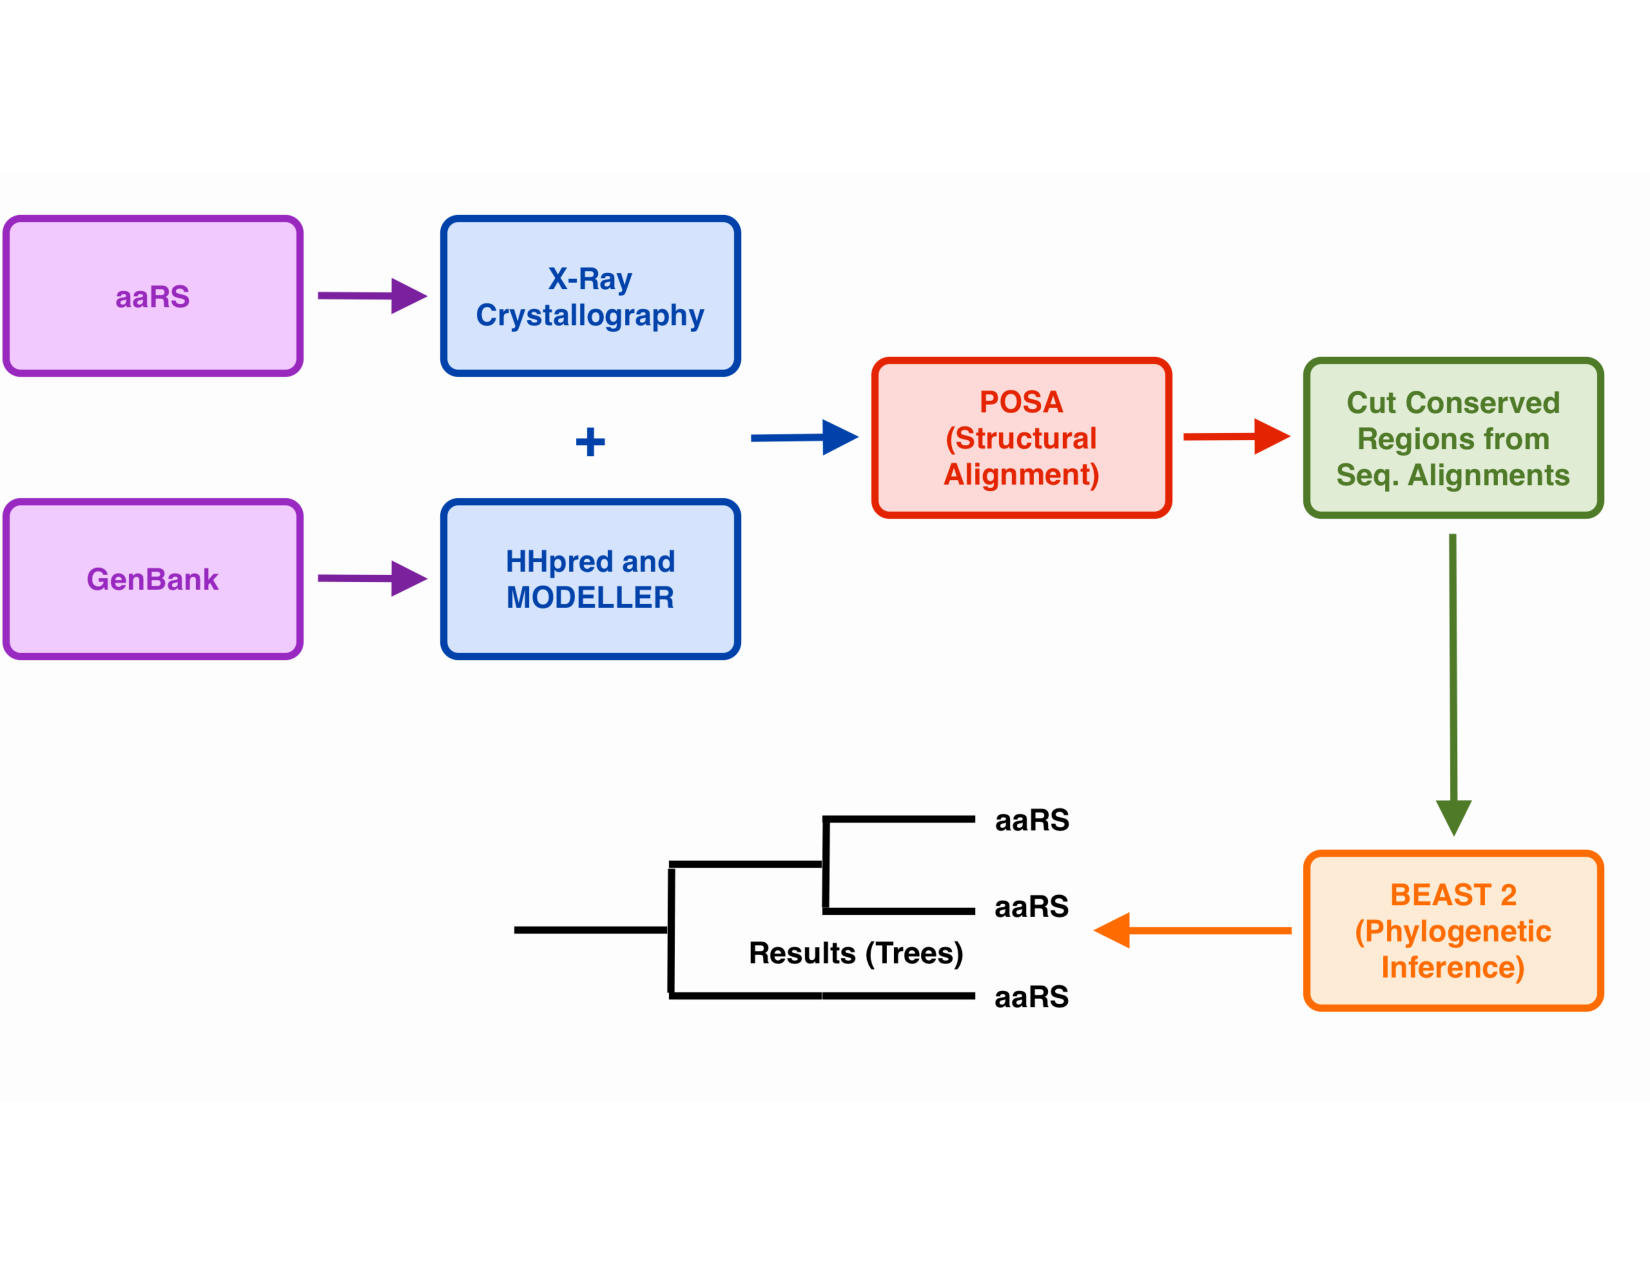
\includegraphics[width=\textwidth]{Pipeline.pdf}
  \label{pipeline}  
\end{figure}

\begin{eqnarray}
\label{eq:schemeP}
%	\mathrm{P_Y} = \underbrace{H(Y_n) - H(Y_n|\mathbf{V}^{Y}_{n})}_{S_Y} + \underbrace{H(Y_n|\mathbf{V}^{Y}_{n})- H(Y_n|\mathbf{V}^{X,Y}_{n})}_{T_{X\rightarrow Y}},
\end{eqnarray}

\section*{Materials and methods}
\subsection*{X-ray crystallography structures}



\subsection*{Modelling structures}
To ensure a statistically significant and diverse dataset, we gathered additional amino acid sequences from GenBank.  
We selected 20 organisms from each of the 3 domains of life, sampling from as many distinct clades as possible along the tips of the tree of life found in Figure \ref{treeoflife} [from: \hyperref[label_name]{``http://tolweb.org/Eukaryotes/3''}]. 
The result of our sampling is shown in Figure \ref{sampledtree}.

We used the ``protein homology detection and protein structure prediction" program HHpred \cite{HHpred} and Modeller \cite{Modeller} to provide 3D structures to the aaRS data from the GenBank database.  
HHpred, which is available through the online server (http://toolkit.tuebingen.mpg.de/\#/) searches the database for known structures that closely match the input queries (i. e., our GenBank sequences).  
It feeds its produced alignment with the known structures to Modeller, which infers structures for the input queries based upon the known structure.

We align the modelled structures with the aaRS structures obtained by x-ray crystallography.  This ensures a more complete dataset.


\begin{figure}
  \caption{\bf Tree of Life.  The tree from which we sampled as broadly as possible.}
  \centering
    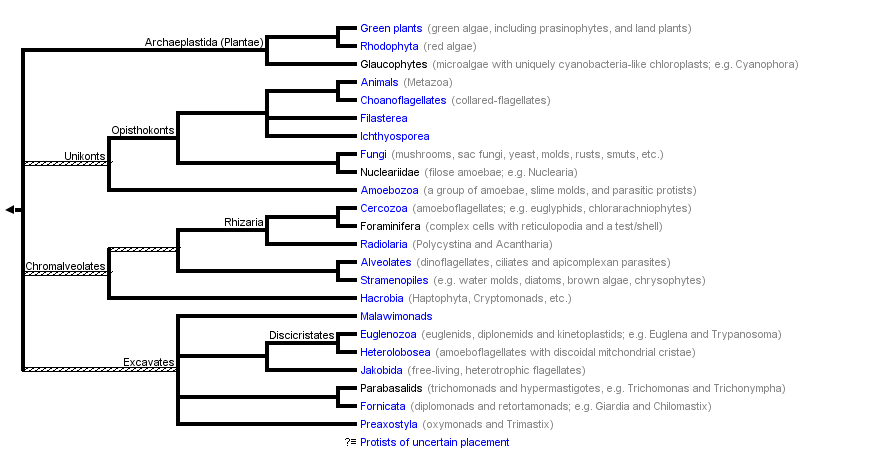
\includegraphics[width=\textwidth]{Eukaryotes.png}
  \label{treeoflife}  
\end{figure}



\subsection*{Structural alignments}


The advantage of Partial Order Structure Alignment (POSA) is that, by utilizing partial order graphs which record one or more possibilities at each position in an alignment, POSA allows for flexibility in the way it estimates structural divergence. \cite{POSA} 
Distinctively, POSA is able to detect conserved regions within a subset of the input structures rather than those which are universally conserved.  In addition, POSA distinguishes internal structural arrangements in the proteins. \cite{POSA} 


Unfortunately, we are unable at this time to perform phylogenetic analysis directly on structural alignments, so to get the POSA alignments into a format we can use, we had to convert the partial order alignments it outputs into simple FASTA files.

A partial order alignment is shown in Figure \ref{POA} [from: ``http://github.com/ekg/glia"].  The difference between this type of alignment and ones used for phylogenetic inference and more typically shown and output by alignment tools is that

\begin{figure}
  \caption{\bf Partial Order Alignment.} This visualisation from ``http://github.com/ekg/glia" shows an alignment as it is normally shown, then a partial order graph applied to sequence alignments.
  \centering
    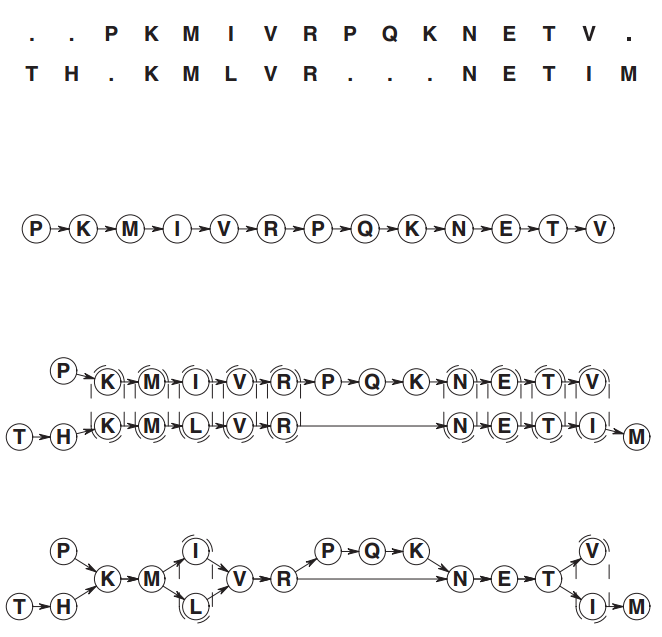
\includegraphics[width=\textwidth]{POA.png}
  \label{POA}  
\end{figure}

\subsection*{Conserved regions}


\subsection*{Phylogenetic inference}

\textit{Bayesian inference}
Based on Bayes' theorem \cite{Bayes}, Bayesian inference supplies straight-forward measures of uncertainty in its posterior probabilities and credible intervals.  
In classical, or frequentist, statistics the premise is that parameters are fixed and data are random.  Therefore, they report confidence intervals, which show a range of values to include the true value of some parameter with a minimum probability (e. g., 95\%).
Bayesians, on the other hand, believe that probability is fundamentally measuring the degree of certainty and thus the parameters are random and the data are fixed. The credible interval is used to denote the range of values that include some percentage (e. g., 95\%) of the probability. \cite{ConfidenceInterval}
In other words, a frequentist designs an experiment to produce a number of trials in which the data (in this case, the sequence data) changes from each trial to the next and then looks for the confidence interval that includes, say, 95\% of the true parameter value (a ``true" tree, or phylogeny, in this case).  
A Bayesian takes the provided (sequence) data as a \textit{given} and then computes probabilities of different parameter values (which describe the possible tree topologies) that could explain the data.
The credible interval, then, is the way to describe how certain or uncertain we are about the answers that were inferred. \cite{PPinBayesianPhylogenetics}

The power of Bayesian statistics in phylogenetics has sparked interest among a growing community of researchers over the years. \cite{Huelsenbeck} \cite{HolderLewis} \cite{MammalRadiation} \cite{EarlyMammals} \cite{MissingData} \cite{SPREAD} \cite{MammalDiversification} \cite{SampledAncestors} \cite{Phylodynamics}
In particular, the Bayesian Evolutionary Analysis by Sampling Trees (BEAST) software provides a framework for relatively easy introduction of new models and parameterizations in its statistical framework for the analysis of countless evolutionary questions. \cite{BEAST} \cite{BEAST1point7} \cite{BEAST2}.
Because of the nature of the Bayesian approach, it permits the ability to incorporate prior knowledge (e. g., past population dynamics) into the inference by using it to generate a prior probability distribution to indicate where the true parameter values probably exist.  
If not much is known previous to the analysis, these things can simply be inferred and the prior distribution is not heavily weighted. \cite{MCMC}

\textit{MCMC}
In order to perform Bayesian inference, one must have a method of sampling the probability distribution.  A popular choice is to implement Metropolis-Hastings Markov chain Monte Carlo (MCMC) integration. \cite{MCMC} \cite{Metropolis} \cite{Hastings}  
The general idea here is that, after sampling one tree, another is proposed that has either higher probability given the sequence data or lower.  The higher probability tree is more readily accepted than the lower probability tree - however, the lower probability tree is sometimes accepted, and in this way it is possible to sample around the distribution and move across low probability ``valleys" to escape local maxima and find the global maximum.  \cite{}

%MCMC efficiency \cite{MCMCefficiency}

\textit{Bayesian phylogenetics} The Bayesian method to phylogenetic inference attempts to obtain a posterior probability distribution of trees Pr($\tau,\theta|D$), where $\tau$ represents the trees sampled, $\theta$ is the substitution model, and $D$ is the data.  In our case, the data is the sequence alignment of amino acids which was produced by structurally aligning the aaRSs.
The prior distributions Pr($\tau|\theta$)Pr($\theta$), which represent the prior knowledge available to the researcher, are combined with the likelihood calculation Pr($D|\tau$).  \cite{PPinBayesianPhylogenetics} The full equation, then is

\begin{eqnarray}
\Pr(\tau,\theta|D) = \frac{\Pr(D|\tau,\theta)\Pr(\tau|\theta)\Pr(\theta)}{\Pr(D)},
\label{eq:posterior}
\end{eqnarray}
where Pr($D$) is a normalization constant which can be ignored.


%\begin{eqnarray}
%\ f(\tree,\traj,\eta, \theta | D) = \frac{\Pr (D|\tree,\theta) f(\tree|\traj,\eta) f(\traj |\eta) f(\eta) f(\theta) }{\Pr(D)},
%\label{eq:posterior}
%\end{eqnarray}

\textit{Molecular Clock}
A strict molecular clock with invariable rates would be inappropriate for our dataset, given the breadth of time our phylogenies span, from present-day stretching all the way to before the divergence of the last universal common ancestor (LUCA) that connects the three domains of life: Archaea, Bacteria, Eukarya. 
We are not particularly interested in the branches near the tips, which distinguish the species, but the fact that the rates of evolution within these branches should be vastly different than those which fixed into populations billions of years in the past cannot be ignored.  Therefore, we chose to use a 
relaxed molecular clock to allow the rate at which mutations fixed into the populations - i. e., the rate of evolution - to vary. \cite{RelaxedClockModelSelection}  With little information to go on concerning the effective population sizes throughout time, we chose a log normal distribution. 

\textit{Population dynamics and tree priors}
Bayesian skyline models yield information about past population dynamics without the need to parameterize with differential equations, and so allow us to estimate the population dynamics rather than making assumptions for which we have limited prior knowledge. \cite{coalSky} \cite{BDSKY}

\textit{Other methods}  There are other methods of analyzing molecular data to infer phylogenies. [CITE CRITICISMS oF BAYES HERE] In maximum likelihood \cite{Guindon}, the likelihood calculation Pr($D|\tau$) is the sole piece of the inference and yields one tree that maximizes the likelihood.  Rather than posterior probabilities, the branches of the tree are labelled with bootstrap values. \cite{HolderLewis}
%Maximum likelihood trees are provided in the Supporting Information.



% Results and Discussion can be combined.
\section*{Results}

The aminoacyl-tRNA synthetases group together in largely expected ways.  The aaRSs which catalyse the attachment of the branched-chain and non-polar amino acids leucine, isoleucine, and valine share a clade within the Class I phylogeny.


% Place tables after the first paragraph in which they are cited.
\begin{table}[!ht]
\scriptsize
\begin{adjustwidth}{-2.66in}{0in} % Comment out/remove adjustwidth environment if table fits in text column.
\centering
\caption{
{\bf Archaea aaRS data sampled and analysed}}
\begin{tabular}{|l+l|l|l|l|l|l|l|l|l|l|l|l|l|l|l|l|l|l|l|l|}
\hline
\multicolumn{1}{|l|}{\bf Organism} & \multicolumn{1}{|l|}{\bf ala} & \multicolumn{1}{|l|}{\bf arg} & \multicolumn{1}{|l|}{\bf asn} & \multicolumn{1}{|l|}{\bf asp} & \multicolumn{1}{|l|}{\bf cys} & \multicolumn{1}{|l|}{\bf gln} & \multicolumn{1}{|l|}{\bf glu} & \multicolumn{1}{|l|}{\bf gly} & \multicolumn{1}{|l|}{\bf his} & \multicolumn{1}{|l|}{\bf ile} & \multicolumn{1}{|l|}{\bf leu} & \multicolumn{1}{|l|}{\bf lys} & \multicolumn{1}{|l|}{\bf met} & \multicolumn{1}{|l|}{\bf phe} & \multicolumn{1}{|l|}{\bf pro} & \multicolumn{1}{|l|}{\bf ser} & \multicolumn{1}{|l|}{\bf thr} & \multicolumn{1}{|l|}{\bf trp} & \multicolumn{1}{|l|}{\bf tyr} & \multicolumn{1}{|l|}{\bf val} \\ \thickhline
$A.\ fulgidus$ & $\Theta$ & $\alpha$ & + & $\alpha$ & $\alpha$ & n/a & $\alpha$ & $\alpha$ & $\alpha$ & $\alpha$ & + & $\alpha$ & $\alpha$ & $\alpha$ & $\alpha$ & $\alpha$ & $\alpha$ & $\alpha$ & $\Theta$ & $\alpha$ \\ \hline
$A.\ pernix$ & $\alpha$ & $\alpha$ & -- & $\alpha$ & $\alpha$ & n/a & $\alpha$ & $\alpha$ & $\alpha$ & $\alpha$ & $\alpha$ & $\alpha$ & $\alpha$ & $\alpha$ & $\alpha$ & $\alpha$ & $\Theta$ & -- & $\Theta$ & $\alpha$ \\ \hline
$Halobacterium\ sp.$ & + & $\alpha$ & + & $\alpha$ & $\alpha$ & n/a & $\alpha$ & $\alpha$ & $\alpha$ & $\alpha$ & + & $\alpha$ & $\alpha$ & $\alpha$ & + & $\alpha$ & $\alpha$ & $\alpha$ & $\alpha$ & $\alpha$ \\ \hline
$M.\ acetivorans$ & $\alpha$ & $\alpha$ & + & $\alpha$ & + & n/a & + & $\alpha$ & $\alpha$ & $\alpha$ & + & $\alpha$ & $\alpha$ & $\alpha$ & $\alpha$ & $\alpha$ & $\alpha$ & $\alpha$ & $\alpha$ & $\alpha$ \\ \hline
$M.\ aeolicus\ Nankai$ & $\alpha$ & $\alpha$ & + & $\alpha$ & + & n/a & + & $\alpha$ & $\alpha$ & + & + & $\alpha$ & $\alpha$ & $\alpha$ & $\alpha$ & $\alpha$ & $\alpha$ & + & $\alpha$ & $\alpha$ \\ \hline
$M.\ barkeri$ & -- & -- & -- & -- & -- & n/a & -- & -- & -- & -- & -- & -- & -- & -- & -- & $\Theta$ & -- & -- & -- & -- \\ \hline
$M.\ hungatei$ & $\alpha$ & $\alpha$ & + & + & $\alpha$ & n/a & $\alpha$ & $\alpha$ & $\alpha$ & $\alpha$ & + & + & $\alpha$ & $\alpha$ & $\alpha$ & $\alpha$ & $\alpha$ & $\alpha$ & $\alpha$ & $\alpha$ \\ \hline
$M.\ jannaschii$ & $\alpha$ & $\alpha$ & + & $\alpha$ & -- & n/a & $\alpha$ & $\alpha$ & $\alpha$ & $\alpha$ & + & -- & $\alpha$ & $\alpha$ & $\Theta$ & $\alpha$ & $\alpha$ & $\alpha$ & $\Theta$ & $\alpha$ \\ \hline
$M.\ kandleri$ & $\alpha$ & $\alpha$ & + & $\alpha$ & + & n/a & $\alpha$ & $\alpha$ & $\alpha$ & $\alpha$ & + & $\alpha$ & $\alpha$ & $\alpha$ & $\alpha$ & $\alpha$ & $\alpha$ & $\alpha$ & $\alpha$ & $\alpha$ \\ \hline
$M.\ thermautotrophicus$ & $\alpha$ & $\alpha$ & + & $\alpha$ & + & n/a & $\alpha$ & $\alpha$ & $\alpha$ & $\alpha$ & $\alpha$ & $\alpha$ & $\alpha$ & $\alpha$ & + & $\alpha$ & $\alpha$ & $\alpha$ & $\alpha$ & $\alpha$ \\ \hline
$N.\ equitans$ & + & $\alpha$ & $\alpha$ & $\alpha$ & $\alpha$ & n/a & + & $\alpha$ & $\alpha$ & $\alpha$ & $\alpha$ & $\alpha$ & $\alpha$ & $\alpha$ & $\alpha$ & $\alpha$ & $\alpha$ & $\alpha$ & $\alpha$ & $\alpha$ \\ \hline
$P.\ abyssi$ & -- & -- & -- & -- & -- & n/a & -- & -- & -- & -- & -- & -- & $\Theta$ & -- & -- & -- & -- & -- & -- & -- \\ \hline
$P.\ aerophilum$ & + & $\alpha$ & $\alpha$ & $\alpha$ & $\alpha$ & n/a & $\alpha$ & $\alpha$ & $\alpha$ & $\alpha$ & $\alpha$ & + & $\alpha$ & $\alpha$ & $\alpha$ & $\alpha$ & $\alpha$ & $\alpha$ & $\alpha$ & $\alpha$ \\ \hline
$P.\ delaneyi$ & $\alpha$ & $\alpha$ & -- & $\alpha$ & $\alpha$ & n/a & $\alpha$ & $\alpha$ & $\alpha$ & $\alpha$ & $\alpha$ & $\alpha$ & $\alpha$ & $\alpha$ & $\alpha$ & $\alpha$ & $\alpha$ & $\alpha$ & $\alpha$ & $\alpha$ \\ \hline
$P.\ horikoshii$ & $\Theta$ & $\Theta$ & $\Theta$ & $\alpha$ & $\alpha$ & n/a & + & $\alpha$ & $\alpha$ & $\alpha$ & $\Theta$ & $\Theta$ & $\alpha$ & $\alpha$ & $\alpha$ & $\alpha$ & $\alpha$ & $\alpha$ & $\Theta$ & $\alpha$ \\ \hline
$P.\ occultum$ & $\alpha$ & $\alpha$ & -- & -- & $\alpha$ & n/a & $\alpha$ & $\alpha$ & $\alpha$ & $\alpha$ & $\alpha$ & $\alpha$ & $\alpha$ & $\alpha$ & $\alpha$ & $\alpha$ & $\alpha$ & $\alpha$ & $\alpha$ & $\alpha$ \\ \hline
$S.\ acidocaldarius$ & $\alpha$ & $\alpha$ & + & $\alpha$ & $\alpha$ & n/a & $\alpha$ & $\alpha$ & $\alpha$ & $\alpha$ & $\alpha$ & + & $\alpha$ & + & $\alpha$ & $\alpha$ & $\alpha$ & $\alpha$ & $\alpha$ & $\alpha$ \\ \hline
$S.\ marinus$ & $\alpha$ & $\alpha$ & $\alpha$ & $\alpha$ & $\alpha$ & n/a & $\alpha$ & $\alpha$ & -- & $\alpha$ & $\alpha$ & $\alpha$ & $\alpha$ & $\alpha$ & $\alpha$ & $\alpha$ & $\alpha$ & + & $\alpha$ & + \\ \hline
$S.\ tokodaii$ & -- & -- & -- & $\Theta$ & -- & n/a & -- & -- & -- & -- & -- & -- & -- & -- & -- & -- & -- & -- & -- & -- \\ \hline
$T.\ acidophilum$ & + & $\alpha$ & $\alpha$ & $\alpha$ & $\alpha$ & n/a & $\alpha$ & $\alpha$ & $\Theta$ & $\alpha$ & $\alpha$ & $\alpha$ & $\alpha$ & + & $\alpha$ & $\alpha$ & $\alpha$ & $\alpha$ & $\alpha$ & $\alpha$ \\ \hline
$T.\ kodakarensis$ & $\alpha$ & $\alpha$ & $\alpha$ & $\Theta$ & $\alpha$ & n/a & $\alpha$ & $\alpha$ & $\alpha$ & $\alpha$ & $\alpha$ & $\alpha$ & $\alpha$ & $\alpha$ & $\alpha$ & $\alpha$ & $\alpha$ & $\alpha$ & $\alpha$ & + \\ \hline
$T.\ volcanium$ & $\alpha$ & + & $\alpha$ & $\alpha$ & + & n/a & $\alpha$ & $\alpha$ & $\alpha$ & $\alpha$ & $\alpha$ & $\alpha$ & $\alpha$ & $\alpha$ & $\alpha$ & $\alpha$ & $\alpha$ & $\alpha$ & $\alpha$ & $\alpha$ \\ \hline
\end{tabular}
\begin{flushleft} \textbf{$\Theta$} means we have the crystal structures for this organism; $\alpha$ means the data was collected from Genbank, successfully modelled, and aligned; + means the data was collected from Genbank but not used in the final alignment; -- means the data was not obtained
\end{flushleft}
\label{table1}
\end{adjustwidth}
\end{table}

\begin{table}[!ht]
\scriptsize
\begin{adjustwidth}{-2.66in}{0in} % Comment out/remove adjustwidth environment if table fits in text column.
\centering
\caption{
{\bf Bacteria aaRS data sampled and analysed}}
\begin{tabular}{|l+l|l|l|l|l|l|l|l|l|l|l|l|l|l|l|l|l|l|l|l|}
\hline
\multicolumn{1}{|l|}{\bf Organism} & \multicolumn{1}{|l|}{\bf ala} & \multicolumn{1}{|l|}{\bf arg} & \multicolumn{1}{|l|}{\bf asn} & \multicolumn{1}{|l|}{\bf asp} & \multicolumn{1}{|l|}{\bf cys} & \multicolumn{1}{|l|}{\bf gln} & \multicolumn{1}{|l|}{\bf glu} & \multicolumn{1}{|l|}{\bf gly} & \multicolumn{1}{|l|}{\bf his} & \multicolumn{1}{|l|}{\bf ile} & \multicolumn{1}{|l|}{\bf leu} & \multicolumn{1}{|l|}{\bf lys} & \multicolumn{1}{|l|}{\bf met} & \multicolumn{1}{|l|}{\bf phe} & \multicolumn{1}{|l|}{\bf pro} & \multicolumn{1}{|l|}{\bf ser} & \multicolumn{1}{|l|}{\bf thr} & \multicolumn{1}{|l|}{\bf trp} & \multicolumn{1}{|l|}{\bf tyr} & \multicolumn{1}{|l|}{\bf val} \\ \thickhline
$A.\ aeolicus$ & $\Theta$ & $\alpha$ & + & $\alpha$ & $\alpha$ & + & + & + & $\alpha$ & $\alpha$ & $\alpha$ & + & $\Theta$ & $\alpha$ & $\alpha$ & $\alpha$ & $\alpha$ & $\alpha$ & $\alpha$ & + \\ \hline
$B.\ burgdorferi$ & $\alpha$ & $\alpha$ & $\alpha$ & $\alpha$ & $\alpha$ & + & $\alpha$ & $\alpha$ & $\alpha$ & $\alpha$ & $\alpha$ & + & $\alpha$ & + & $\alpha$ & $\alpha$ & $\alpha$ & $\alpha$ & $\alpha$ & $\alpha$ \\ \hline
$B.\ fragilis$ & $\alpha$ & $\alpha$ & $\alpha$ & $\alpha$ & $\alpha$ & $\alpha$ & $\alpha$ & $\alpha$ & $\alpha$ & $\alpha$ & + & $\alpha$ & $\alpha$ & + & $\alpha$ & $\alpha$ & $\alpha$ & $\alpha$ & $\alpha$ & + \\ \hline
$B.\ licheniformis$ & $\alpha$ & $\alpha$ & + & $\alpha$ & $\alpha$ & + & $\alpha$ & + & $\alpha$ & $\alpha$ & $\alpha$ & $\alpha$ & $\alpha$ & $\alpha$ & $\alpha$ & $\alpha$ & $\alpha$ & $\alpha$ & $\alpha$ & $\alpha$ \\ \hline
$B.\ thailandensis$ & $\alpha$ & $\alpha$ & + & $\alpha$ & $\alpha$ & $\alpha$ & $\alpha$ & $\alpha$ & $\alpha$ & $\alpha$ & $\alpha$ & $\alpha$ & $\alpha$ & $\alpha$ & $\alpha$ & $\alpha$ & + & $\alpha$ & + & $\alpha$ \\ \hline
$C.\ A.\ asiaticus$ & $\alpha$ & $\alpha$ & $\alpha$ & $\alpha$ & $\alpha$ & + & + & $\alpha$ & $\alpha$ & $\alpha$ & $\alpha$ & $\alpha$ & $\alpha$ & $\alpha$ & $\alpha$ & $\alpha$ & $\alpha$ & $\alpha$ & $\alpha$ & $\alpha$ \\ \hline
$C.\ aggregans$ & $\alpha$ & $\alpha$ & $\alpha$ & $\alpha$ & $\alpha$ & + & $\alpha$ & $\alpha$ & $\alpha$ & $\alpha$ & $\alpha$ & $\alpha$ & $\alpha$ & $\alpha$ & $\alpha$ & $\alpha$ & $\alpha$ & $\alpha$ & $\alpha$ & + \\ \hline
$C.\ jejuni$ & + & $\Theta$ & + & $\alpha$ & $\alpha$ & $\alpha$ & $\alpha$ & + & $\alpha$ & $\alpha$ & $\alpha$ & $\alpha$ & $\alpha$ & $\alpha$ & + & $\alpha$ & $\alpha$ & $\alpha$ & $\alpha$ & $\alpha$ \\ \hline
$C.\ thermalis$ & $\alpha$ & $\alpha$ & $\alpha$ & + & $\alpha$ & + & + & + & $\alpha$ & $\alpha$ & $\alpha$ & + & $\alpha$ & $\alpha$ & $\alpha$ & $\alpha$ & $\alpha$ & $\alpha$ & $\alpha$ & $\alpha$ \\ \hline
$D.\ radiodurans$ & $\alpha$ & $\alpha$ & $\alpha$ & $\alpha$ & $\alpha$ & $\Theta$ & $\alpha$ & $\alpha$ & $\alpha$ & $\alpha$ & $\alpha$ & $\alpha$ & $\alpha$ & $\alpha$ & $\alpha$ & $\alpha$ & $\alpha$ & $\alpha$ & $\alpha$ & $\alpha$ \\ \hline
$E.\ coli$ & $\Theta$ & $\alpha$ & $\alpha$ & $\Theta$ & $\Theta$ & $\Theta$ & $\Theta$ & $\Theta$ & $\Theta$ & $\alpha$ & $\alpha$ & $\Theta$ & $\Theta$ & $\alpha$ & $\alpha$ & $\alpha$ & $\Theta$ & $\alpha$ & $\Theta$ & $\alpha$ \\ \hline
$E.\ faecalis$ & $\alpha$ & $\alpha$ & $\alpha$ & $\alpha$ & $\alpha$ & -- & $\alpha$ & $\alpha$ & $\alpha$ & $\alpha$ & $\alpha$ & $\alpha$ & $\alpha$ & $\alpha$ & $\Theta$ & $\alpha$ & $\alpha$ & $\alpha$ & $\alpha$ & $\alpha$ \\ \hline
$G.\ obscuriglobus$ & $\alpha$ & $\alpha$ & $\alpha$ & + & $\alpha$ & $\alpha$ & $\alpha$ & $\alpha$ & $\alpha$ & $\alpha$ & $\alpha$ & $\alpha$ & $\alpha$ & $\alpha$ & $\alpha$ & + & $\alpha$ & $\alpha$ & $\alpha$ & + \\ \hline
$G.\ stearothermophilus$ & $\alpha$ & $\alpha$ & + & $\alpha$ & + & $\alpha$ & $\alpha$ & $\alpha$ & $\alpha$ & $\alpha$ & $\alpha$ & $\Theta$ & $\alpha$ & -- & $\alpha$ & $\alpha$ & $\alpha$ & $\Theta$ & $\alpha$ & $\alpha$ \\ \hline
$H.\ aurantiacus$ & $\alpha$ & $\alpha$ & $\alpha$ & $\alpha$ & $\alpha$ & -- & $\alpha$ & $\alpha$ & $\alpha$ & $\alpha$ & + & $\alpha$ & $\alpha$ & $\alpha$ & $\alpha$ & $\alpha$ & $\alpha$ & $\alpha$ & $\alpha$ & + \\ \hline
$M.\ mobile$ & $\alpha$ & + & $\alpha$ & $\alpha$ & $\alpha$ & -- & $\Theta$ & $\alpha$ & $\alpha$ & $\alpha$ & $\alpha$ & $\alpha$ & + & $\alpha$ & + & $\alpha$ & + & + & $\alpha$ & $\alpha$ \\ \hline
$M.\ smegmatis$ & + & + & + & $\alpha$ & $\Theta$ & + & + & + & + & + & $\alpha$ & + & $\alpha$ & $\alpha$ & + & $\alpha$ & + & + & + & $\alpha$ \\ \hline
$P.\ mikurensis$ & $\alpha$ & $\alpha$ & -- & $\alpha$ & $\alpha$ & $\alpha$ & $\alpha$ & $\alpha$ & $\alpha$ & $\alpha$ & + & $\alpha$ & $\alpha$ & $\alpha$ & $\alpha$ & + & $\alpha$ & $\alpha$ & $\alpha$ & + \\ \hline
$R.\ marinus$ & + & $\alpha$ & $\alpha$ & $\alpha$ & $\alpha$ & -- & $\alpha$ & $\alpha$ & $\alpha$ & $\alpha$ & + & + & $\alpha$ & $\alpha$ & $\alpha$ & $\alpha$ & $\alpha$ & $\alpha$ & * & $\alpha$ \\ \hline
$R.\ palustris$ & $\alpha$ & $\alpha$ & -- & $\alpha$ & $\alpha$ & $\alpha$ & + & $\alpha$ & $\alpha$ & + & + & $\alpha$ & $\alpha$ & $\alpha$ & $\Theta$ & $\alpha$ & $\alpha$ & $\alpha$ & $\alpha$ & $\alpha$ \\ \hline
$S.\ aureus$ & $\alpha$ & $\alpha$ & $\alpha$ & $\alpha$ & $\alpha$ & + & + & $\Theta$ & $\Theta$ & $\Theta$ & $\alpha$ & $\alpha$ & $\alpha$ & $\alpha$ & $\alpha$ & $\alpha$ & $\Theta$ & $\alpha$ & $\Theta$ & $\alpha$ \\ \hline
$S.\ elongatus$ & $\alpha$ & $\alpha$ & $\alpha$ & $\alpha$ & $\alpha$ & $\alpha$ & $\Theta$ & $\alpha$ & $\alpha$ & $\alpha$ & $\alpha$ & $\alpha$ & $\alpha$ & + & $\alpha$ & $\alpha$ & $\alpha$ & $\alpha$ & $\alpha$ & $\alpha$ \\ \hline
$S.\ haemolyticus$ & $\alpha$ & $\alpha$ & $\alpha$ & $\alpha$ & $\alpha$ & -- & $\alpha$ & $\alpha$ & $\alpha$ & $\alpha$ & $\alpha$ & $\alpha$ & $\alpha$ & $\Theta$ & $\alpha$ & $\alpha$ & $\alpha$ & $\alpha$ & $\alpha$ & $\alpha$ \\ \hline
$S.\ typhimurium$ & -- & -- & -- & -- & -- & -- & -- & -- & -- & -- & -- & $\Theta$ & -- & -- & -- & -- & -- & -- & -- & -- \\ \hline
$T.\ maritima$ & $\alpha$ & $\alpha$ & + & $\alpha$ & $\alpha$ & $\Theta$ & $\Theta$ & $\Theta$ & $\alpha$ & $\alpha$ & $\alpha$ & $\alpha$ & $\alpha$ & -- & $\alpha$ & $\alpha$ & $\alpha$ & $\Theta$ & $\alpha$ & $\alpha$ \\ \hline
$T.\ thermophilus$ & $\alpha$ & $\Theta$ & $\Theta$ & $\Theta$ & $\alpha$ & $\Theta$ & $\Theta$ & $\Theta$ & $\Theta$ & $\Theta$ & $\Theta$ & $\alpha$ & $\Theta$ & $\Theta$ & $\Theta$ & $\Theta$ & $\alpha$ & $\Theta$ & $\Theta$ & $\Theta$ \\ \hline
\end{tabular}
\begin{flushleft} \textbf{$\Theta$} means we have the crystal structures for this organism; $\alpha$ means the data was collected from Genbank, successfully modelled, and aligned; + means the data was collected from Genbank but not used in the final alignment; -- means the data was not obtained
\end{flushleft}
\label{table1}
\end{adjustwidth}
\end{table}

\begin{table}[!ht]
\scriptsize
\begin{adjustwidth}{-2.56in}{0in} % Comment out/remove adjustwidth environment if table fits in text column.
\centering
\caption{
{\bf Eukaryote aaRS data sampled and analysed}}
\begin{tabular}{|l+l|l|l|l|l|l|l|l|l|l|l|l|l|l|l|l|l|l|l|l|}
\hline
\multicolumn{1}{|l|}{\bf Organism} & \multicolumn{1}{|l|}{\bf ala} & \multicolumn{1}{|l|}{\bf arg} & \multicolumn{1}{|l|}{\bf asn} & \multicolumn{1}{|l|}{\bf asp} & \multicolumn{1}{|l|}{\bf cys} & \multicolumn{1}{|l|}{\bf gln} & \multicolumn{1}{|l|}{\bf glu} & \multicolumn{1}{|l|}{\bf gly} & \multicolumn{1}{|l|}{\bf his} & \multicolumn{1}{|l|}{\bf ile} & \multicolumn{1}{|l|}{\bf leu} & \multicolumn{1}{|l|}{\bf lys} & \multicolumn{1}{|l|}{\bf met} & \multicolumn{1}{|l|}{\bf phe} & \multicolumn{1}{|l|}{\bf pro} & \multicolumn{1}{|l|}{\bf ser} & \multicolumn{1}{|l|}{\bf thr} & \multicolumn{1}{|l|}{\bf trp} & \multicolumn{1}{|l|}{\bf tyr} & \multicolumn{1}{|l|}{\bf val} \\ \thickhline
$A.\ subglabra$ & -- & $\alpha$ & $\alpha$ & $\alpha$ & -- & $\alpha$ & $\alpha$ & $\alpha$ & $\alpha$ & $\alpha$ & $\alpha$ & $\alpha$ & $\alpha$ & + & $\alpha$ & $\alpha$ & $\alpha$ & $\alpha$ & $\alpha$ & -- \\ \hline
$B.\ hominis$ & $\alpha$ & -- & -- & $\alpha$ & $\alpha$ & -- & $\alpha$ & $\alpha$ & -- & $\alpha$ & $\alpha$ & $\alpha$ & $\alpha$ & $\alpha$ & $\alpha$ & -- & -- & -- & $\alpha$ & $\alpha$ \\ \hline
$B.\ mori$ & $\alpha$ & $\Theta$ & $\alpha$ & $\alpha$ & -- & -- & $\alpha$ & $\alpha$ & -- & $\alpha$ & -- & $\alpha$ & $\alpha$ & $\alpha$ & + & $\alpha$ & $\alpha$ & $\alpha$ & -- & -- \\ \hline
$B.\ taurus$ & + & + & + & -- & + & -- & + & + & + & + & $\alpha$ & + & + & + & + & $\Theta$ & + & $\alpha$ & + & + \\ \hline
$C.\ gigas$ & $\alpha$ & + & $\alpha$ & $\alpha$ & $\alpha$ & $\alpha$ & + & $\alpha$ & $\alpha$ & $\alpha$ & $\alpha$ & $\alpha$ & $\alpha$ & $\alpha$ & $\alpha$ & $\alpha$ & $\alpha$ & $\alpha$ & $\alpha$ & $\alpha$ \\ \hline
$C.\ owczarzaki$ & $\alpha$ & $\alpha$ & $\alpha$ & $\alpha$ & $\alpha$ & $\alpha$ & + & $\alpha$ & $\alpha$ & $\alpha$ & $\alpha$ & $\alpha$ & + & + & $\alpha$ & $\alpha$ & $\alpha$ & $\alpha$ & $\alpha$ & $\alpha$ \\ \hline
$C.\ parvum\ Iowa\ II$ & $\alpha$ & -- & $\alpha$ & $\alpha$ & $\alpha$ & $\alpha$ & $\alpha$ & $\alpha$ & $\alpha$ & $\alpha$ & -- & $\alpha$ & $\alpha$ & + & $\alpha$ & $\alpha$ & + & $\alpha$ & $\alpha$ & $\alpha$ \\ \hline
$C.\ subellipsoidea$ & $\alpha$ & $\alpha$ & + & $\alpha$ & -- & $\alpha$ & -- & $\alpha$ & + & $\alpha$ & $\alpha$ & $\alpha$ & $\alpha$ & + & $\alpha$ & $\alpha$ & $\alpha$ & + & $\alpha$ & $\alpha$ \\ \hline
$D.\ discoideum$ & $\alpha$ & $\alpha$ & $\alpha$ & $\alpha$ & $\alpha$ & -- & + & $\alpha$ & $\alpha$ & $\alpha$ & + & $\alpha$ & $\alpha$ & $\alpha$ & $\alpha$ & $\alpha$ & $\alpha$ & $\alpha$ & $\alpha$ & $\alpha$ \\ \hline
$D.\ rerio$ & $\alpha$ & $\alpha$ & + & -- & + & $\alpha$ & $\alpha$ & + & $\alpha$ & + & + & -- & + & + & + & + & + & $\alpha$ & + & $\alpha$ \\ \hline
$E.\ guttata$ & $\alpha$ & + & + & $\alpha$ & $\alpha$ & $\alpha$ & $\alpha$ & -- & $\alpha$ & $\alpha$ & $\alpha$ & + & $\alpha$ & $\alpha$ & $\alpha$ & $\alpha$ & $\alpha$ & $\alpha$ & + & $\alpha$ \\ \hline
$E.\ histolytica$ & $\alpha$ & + & $\Theta$ & $\Theta$ & $\alpha$ & $\alpha$ & $\alpha$ & $\alpha$ & $\alpha$ & $\alpha$ & + & -- & $\alpha$ & $\alpha$ & $\alpha$ & $\alpha$ & $\alpha$ & $\alpha$ & $\alpha$ & $\alpha$ \\ \hline
$G.\ lamblia$ & + & $\alpha$ & $\alpha$ & $\alpha$ & $\alpha$ & $\alpha$ & -- & $\alpha$ & $\alpha$ & $\alpha$ & $\alpha$ & $\alpha$ & $\alpha$ & $\alpha$ & $\Theta$ & $\alpha$ & $\alpha$ & $\alpha$ & $\alpha$ & $\alpha$ \\ \hline
$G.\ theta$ & $\alpha$ & $\alpha$ & $\alpha$ & $\alpha$ & $\alpha$ & $\alpha$ & + & $\alpha$ & $\alpha$ & $\alpha$ & $\alpha$ & $\alpha$ & $\alpha$ & $\alpha$ & $\alpha$ & $\alpha$ & $\alpha$ & $\alpha$ & $\alpha$ & + \\ \hline
$H.\ sapiens$ & + & + & $\alpha$ & -- & -- & $\Theta$ & $\alpha$ & $\Theta$ & $\alpha$ & $\alpha$ & $\alpha$ & $\Theta$ & $\alpha$ & $\Theta$ & + & $\alpha$ & $\alpha$ & $\Theta$ & $\alpha$ & -- \\ \hline
$L.\ infantum$ & $\alpha$ & $\alpha$ & $\alpha$ & $\alpha$ & $\alpha$ & $\alpha$ & $\alpha$ & $\alpha$ & $\alpha$ & $\alpha$ & $\alpha$ & $\alpha$ & $\alpha$ & $\alpha$ & $\alpha$ & $\alpha$ & $\alpha$ & $\alpha$ & $\alpha$ & $\alpha$ \\ \hline
$M.\ domestica$ & + & $\alpha$ & + & + & + & $\alpha$ & + & + & $\alpha$ & + & + & + & + & $\alpha$ & + & + & + & $\alpha$ & $\alpha$ & $\alpha$ \\ \hline
$N.\ ceranae$ & $\alpha$ & $\alpha$ & $\alpha$ & $\alpha$ & $\alpha$ & $\alpha$ & $\alpha$ & $\alpha$ & + & $\alpha$ & $\alpha$ & $\alpha$ & $\alpha$ & + & $\alpha$ & $\alpha$ & $\alpha$ & $\alpha$ & $\alpha$ & $\alpha$ \\ \hline
$N.\ gruberi$ & $\alpha$ & -- & $\alpha$ & $\alpha$ & $\alpha$ & -- & -- & $\alpha$ & -- & $\alpha$ & + & $\alpha$ & $\alpha$ & $\alpha$ & $\alpha$ & $\alpha$ & $\alpha$ & $\alpha$ & $\alpha$ & $\alpha$ \\ \hline
$P.\ bivittatus$ & + & + & + & + & $\alpha$ & + & + & + & + & + & + & + & + & + & + & + & -- & + & + & + \\ \hline
$P.\ chromatophora$ & $\alpha$ & $\alpha$ & -- & $\alpha$ & $\alpha$ & -- & $\alpha$ & + & $\alpha$ & $\alpha$ & $\alpha$ & $\alpha$ & $\alpha$ & $\alpha$ & $\alpha$ & $\alpha$ & $\alpha$ & $\alpha$ & $\alpha$ & $\alpha$ \\ \hline
$P.\ euphratica$ & + & $\alpha$ & $\alpha$ & -- & + & + & -- & -- & + & + & + & + & + & + & + & + & + & + & + & + \\ \hline
$S.\ cerevisiae$ & -- & $\Theta$ & -- & -- & -- & -- & -- & -- & -- & -- & -- & -- & -- & -- & -- & -- & -- & $\Theta$ & $\Theta$ & -- \\ \hline
$S.\ rosetta$ & $\alpha$ & $\alpha$ & $\alpha$ & $\alpha$ & $\alpha$ & $\alpha$ & $\alpha$ & $\alpha$ & -- & $\alpha$ & + & $\alpha$ & $\alpha$ & $\alpha$ & $\alpha$ & $\alpha$ & $\alpha$ & + & $\alpha$ & $\alpha$ \\ \hline
$R.\ filosa$ & + & -- & + & -- & + & + & + & + & -- & -- & + & + & + & $\alpha$ & $\alpha$ & + & $\alpha$ & + & -- & -- \\ \hline
$T.\ brucei$ & -- & -- & -- & -- & -- & -- & -- & -- & $\Theta$ & -- & -- & + & + & -- & -- & -- & -- & + & + & -- \\ \hline
$T.\ cruzi$ & -- & -- & -- & -- & -- & -- & -- & -- & $\Theta$ & -- & -- & -- & -- & -- & -- & -- & -- & -- & -- & -- \\ \hline
$T.\ vaginalis$ & + & -- & $\alpha$ & -- & $\alpha$ & $\alpha$ & $\alpha$ & $\alpha$ & $\alpha$ & $\alpha$ & $\alpha$ & $\alpha$ & -- & $\alpha$ & $\alpha$ & $\alpha$ & $\alpha$ & $\alpha$ & -- & + \\ \hline
\end{tabular}
\begin{flushleft} \textbf{$\Theta$} means we have the crystal structures for this organism; $\alpha$ means the data was collected from Genbank, successfully modelled, and aligned; + means the data was collected from Genbank but not used in the final alignment; -- means the data was not obtained
\end{flushleft}
\label{table1}
\end{adjustwidth}
\end{table}

% T. BRUCEI TYR/MET???



% Place tables after the first paragraph in which they are cited.
\begin{table}[!ht]
\begin{adjustwidth}{-2.66in}{0in} % Comment out/remove adjustwidth environment if table fits in text column.
\centering
\caption{
{\bf Properties of the amino acids associated with Class I aaRSs}}
\begin{tabular}{|l+l|l|l|l|l|l|l|l|l|l|l|l|l|l|l|l|l|l|l|l|}
\hline
\multicolumn{1}{|l|}{\bf Amino acid} & \multicolumn{1}{|l|}{\bf arg} & \multicolumn{1}{|l|}{\bf cys} & \multicolumn{1}{|l|}{\bf gln} & \multicolumn{1}{|l|}{\bf glu} & \multicolumn{1}{|l|}{\bf ile} & \multicolumn{1}{|l|}{\bf leu} & \multicolumn{1}{|l|}{\bf met} & \multicolumn{1}{|l|}{\bf trp} & \multicolumn{1}{|l|}{\bf tyr} & \multicolumn{1}{|l|}{\bf val} \\ \thickhline
Polar (P) or Non-polar (--) & -- & P & P & -- & -- & -- & -- & P & P & -- \\ \hline
%Side chain (S) &  &  &  &  &  &  &  &  &  & \\ \hline
%$\alpha$-amino group ($\alpha$) &  &  &  &  &  &  &  &  &  &  \\ \hline
%$\alpha$-carboxylic acid group (-COO-) &  &  &  &  &  &  &  &  &  &  \\ \hline
Aromatic (R) or Aliphatic (L) & -- & -- & -- & -- & -- & -- & -- & R & R & -- \\ \hline
Charged (+) or Uncharged (--) & + & -- & -- & + & -- & -- & -- & -- & -- & -- \\ \hline
Hydrophobic (H) or Hydrophilic (--) & -- & -- & -- & -- & H & H & H & -- & -- & H \\ \hline
\end{tabular}
\begin{flushleft} %blah
\end{flushleft}
\label{table2}
\end{adjustwidth}
\end{table}

% Place tables after the first paragraph in which they are cited.
\begin{table}[!ht]
\begin{adjustwidth}{-2.66in}{0in} % Comment out/remove adjustwidth environment if table fits in text column.
\centering
\caption{
{\bf Properties of the amino acids associated with Class II aaRSs}}
\begin{tabular}{|l+l|l|l|l|l|l|l|l|l|l|l|l|l|l|l|l|l|l|l|l|}
\hline
\multicolumn{1}{|l|}{\bf Amino acid} & \multicolumn{1}{|l|}{\bf ala} & \multicolumn{1}{|l|}{\bf asn} & \multicolumn{1}{|l|}{\bf asp} & \multicolumn{1}{|l|}{\bf gly} & \multicolumn{1}{|l|}{\bf his} & \multicolumn{1}{|l|}{\bf lys} & \multicolumn{1}{|l|}{\bf phe} & \multicolumn{1}{|l|}{\bf pro} & \multicolumn{1}{|l|}{\bf ser} & \multicolumn{1}{|l|}{\bf thr} \\ \thickhline
Polar (P) or Non-polar (--) & -- & P & -- & -- & P & -- & -- & -- & P & P \\ \hline
%Side chain (S) & S & S & S &  &  &  &  &  &  & \\ \hline
%$\alpha$-amino group ($\alpha$) & $\alpha$ & $\alpha$ & $\alpha$ &  &  &  &  &  &  & \\ \hline
%$\alpha$-carboxylic acid group (-COO-) & -COO- & -COO- & -COO- &  &  &  &  &  &  & \\ \hline
Aromatic (R) or Aliphatic (--) & -- & -- & -- & -- & R & -- & R & -- & -- & -- \\ \hline
Charged (+) or Uncharged (--) & -- & -- & + & -- & -- & + & -- & -- & -- & -- \\ \hline
Hydrophobic (H) or Hydrophilic (--) & H & -- & -- & H/-- & -- & -- & H & H & -- & -- \\ \hline
\end{tabular}
\begin{flushleft} %blah
\end{flushleft}
\label{table2}
\end{adjustwidth}
\end{table}


%PLOS does not support heading levels beyond the 3rd (no 4th level headings).
\subsection*{\lorem\ and \ipsum\ nunc blandit a tortor}
\subsubsection*{3rd level heading} 


\section*{Discussion}
Nulla mi mi, venenatis sed ipsum varius, Table~\ref{table1} 

\section*{Conclusion}

%CO\textsubscript{2} Maecenas convallis mauris sit amet sem ultrices gravida.  Quisque augue sem, tincidunt sit amet feugiat eget, ullamcorper sed velit. 

Sed non aliquet felis. , see \nameref{S1_Appendix}.

\section*{Supporting information}

Here we provide details of the organisms we sampled for the aaRS Class I and Class II phylogenies.

\begin{figure}
  \caption{\bf Tree of Life.  Tree showing our sampling efficacy.}
  \centering
    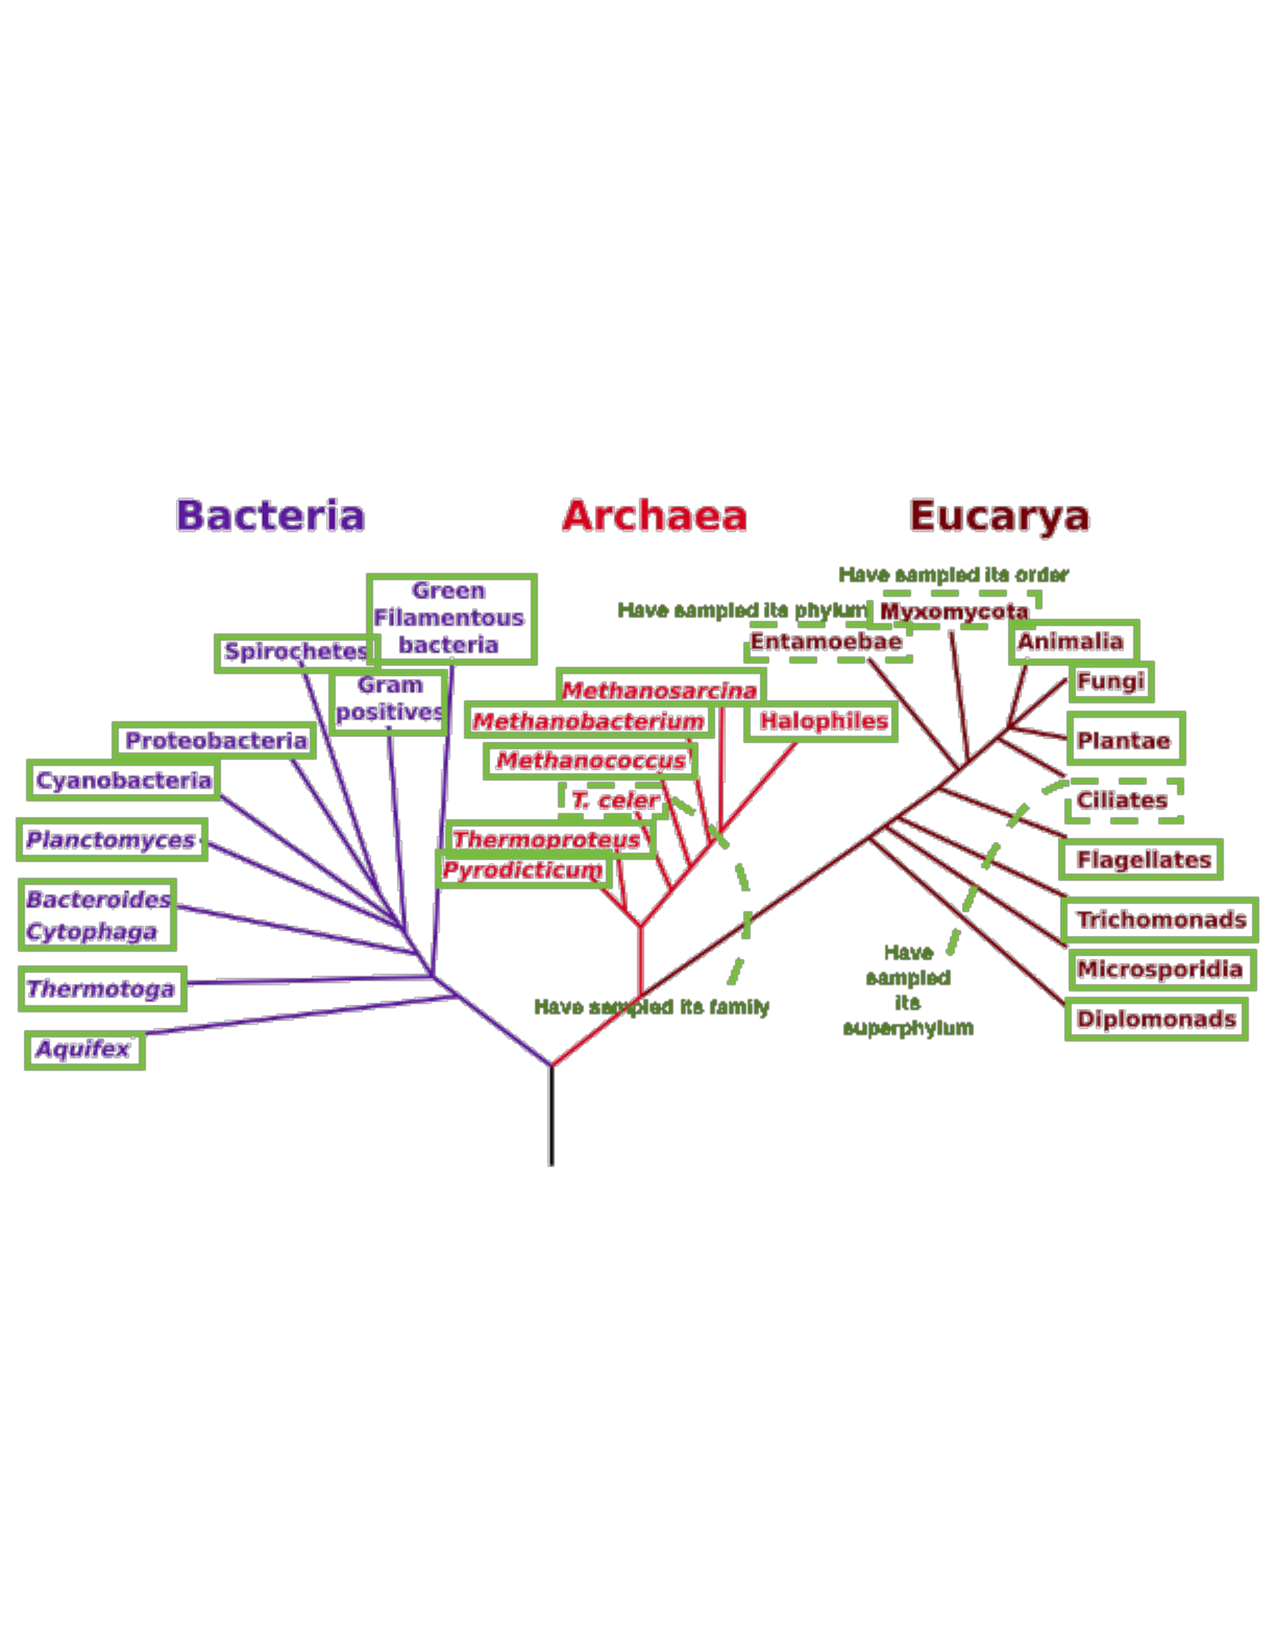
\includegraphics[width=\textwidth]{TreeofLife.pdf}
  \label{sampledtree}  
\end{figure}

Archaea

\begin{itemize}
	\item Methanosarcina
	\begin{itemize}
		\item \textit{Methanosarcina acetivorans}
		\item \textit{Methanosarcina barkeri}
	\end{itemize}
	\item Halophiles
	\begin{itemize}
		\item \textit{Halobacterium sp.}
	\end{itemize}
	\item Methanobacterium
	\begin{itemize}
		\item \textit{Methanothermobacter thermautotrophicus}
	\end{itemize}
	\item Methanococcus
	\begin{itemize}
		\item \textit{Methanococcus aeolicus Nankai}
		\item \textit{Methanococcus jannaschii}
	\end{itemize}
	\item Thermococcus
	\begin{itemize}
		\item \textit{Pyrococcus horikoshii}
		\item \textit{Pyrococcus abyssi}
		\item \textit{Thermococcus kodakarensis}
	\end{itemize}
	\item Thermoproteus
	\begin{itemize}
		\item \textit{Pyrobaculum aerophilum}
		\item \textit{Staphylothermus marinus}
		\item \textit{Sulfolobus acidocaldarius}
		\item \textit{Aeropyrum pernix}
		\item \textit{Sulfolobus tokodaii}
	\end{itemize}
	\item Pyrodicticum
	\begin{itemize}
		\item \textit{Pyrodictium occultum}
		\item \textit{Pyrodictium delaneyi}
	\end{itemize}
	\item Other
	\begin{itemize}
		\item \textit{Methanospirillum hungatei}
		\item \textit{Nanoarchaeum equitans}
		\item \textit{Thermoplasma volcanium}
		\item \textit{Thermoplasma acidophilum}
		\item \textit{Methanopyrus kandleri}
		\item \textit{Archaeoglobus fulgidus}
	\end{itemize}
\end{itemize}

Bacteria

\begin{itemize}
	\item ``Green filamentous bacteria''
	\begin{itemize}
		\item \textit{Chloroflexus aggregans}
		\item \textit{Herpetosiphon aurantiacus}
	\end{itemize}
	\item Gram positives
	\begin{itemize}
		\item \textit{Bacillus licheniformis}
		\item \textit{Geobacillus stearothermophilus}
		\item \textit{Mycobacterium smegmatis}
		\item \textit{Mycoplasma mobile}
		\item \textit{Staphylococcus aureus}
	\end{itemize}
	\item Spirochetes
	\begin{itemize}
		\item \textit{Borrelia burgdorferi}
	\end{itemize}
	\item Proteobacteria
	\begin{itemize}
		\item \textit{Burkholderia thailandensis}
		\item \textit{Campylobacter jejuni}
		\item \textit{Escherichia coli}
		\item \textit{Rhodopseudomonas palustris}
		\item \textit{Salmonella typhimurium}
	\end{itemize}
	\item Cyanobacteria
	\begin{itemize}
		\item \textit{Synechococcus elongatus}
		\item \textit{Chroococcidiopsis thermalis}
	\end{itemize}
	\item Plantomycetes
	\begin{itemize}
		\item \textit{Phycisphaera mikurensis}
		\item \textit{Gemmata obscuriglobus}
	\end{itemize}
	\item Bacteroides/Cytophaga
	\begin{itemize}
		\item \textit{Candidatus Amoebophilus asiaticus}
		\item \textit{Bacteroides fragilis}
	\end{itemize}
	\item Thermotoga
	\begin{itemize}
		\item \textit{Thermotoga maritima}
	\end{itemize}
	\item Aquifex
	\begin{itemize}
		\item \textit{Aquifex aeolicus}
	\end{itemize}
	\item Other
	\begin{itemize}
		\item \textit{Deinococcus radiodurans}
		\item \textit{Thermus thermophilus}
		\item \textit{Enterococcus faecalis}
		\item \textit{Rhodothermus marinus}
		\item \textit{Staphylococcus haemolyticus}
	\end{itemize}
\end{itemize}


Eukarya

\begin{itemize}
	\item Entamoebae/Myxomycota
	\begin{itemize}
		\item \textit{Dictyostelium discoideum} (soil-living amoeba, slime mold)
		\item \textit{Entamoeba histolytica} (anaerobic parasitic amoebozoa)
	\end{itemize}
	\item Animalia
	\begin{itemize}
		\item \textit{Homo sapiens} (human)
		\item \textit{Bos taurus} (cattle)
		\item \textit{Danio rerio} (zebrafish)
		\item \textit{Python bivittatus} (Burmese python)
		\item \textit{Bombyx mori} (silkworm)
		\item \textit{Musca domestica} (housefly)
		\item \textit{Crassostrea gigas} (Pacific oyster)
	\end{itemize}
	\item Fungi
	\begin{itemize}
		\item \textit{Auricularia subglabra} (jelly fungi)
		\item \textit{Saccharomyces cerevisiae} (yeast)
	\end{itemize}
	\item Plantae
	\begin{itemize}
		\item \textit{Erythranthe guttata} (yellow monkey flower)
		\item \textit{Populus euphratica} (Euphrates or desert poplar)
		\item Green algae
		\begin{itemize}
			\item \textit{Coccomyxa subellipsoidea} (green algae)
		\end{itemize}
	\end{itemize}
	\item Ciliates
	\begin{itemize}
		\item \textit{Cryptosporidium parvum Iowa II} (apicomplexan protozoan)
	\end{itemize}
	\item Flagellates
	\begin{itemize}
			\item \textit{Guillardia theta} (flagellate cryptomonad algae)
			\item \textit{Salpingoeca rosetta} (choanoflagellate, closest living relatives of the animals)
			\item \textit{Leishmania infantum} (kinetoplastid protozoan with single flagellum)
			\item Diplomonads
			\begin{itemize}
				\item \textit{Giardia lamblia} (flagellated protozoan parasite)
			\end{itemize}
			\item Trichomonads
			\begin{itemize}
				\item \textit{Trichomonas vaginalis} (anaerobic, flagellated protozoan parasite)
			\end{itemize}
	\end{itemize}
	\item Microsporidia
	\begin{itemize}
		\item \textit{Nosema ceranae} (unicellular honey bee parasite)
	\end{itemize}
	\item Etc.
	\begin{itemize}
		\item \textit{Naegleria gruberi} (famous for ability to change from amoeba to flagellate)
		\item \textit{Blastocystis hominis} (single-celled protozoan human parasite)
		\item \textit{Reticulomyxa filosa} (freshwater foraminifer with anastamozing pseudopodia)
		\item \textit{Capsaspora owczarzaki} (single-celled amoeba symbiont with tropical freshwater snail)
		\item \textit{Paulinella chromatophora} (photosynthetic freshwater amoeba)
		\item \textit{Trypanosoma brucei} (parasite, causes sleeping sickness)
		\item \textit{Trypanosoma cruzi} (parasite, causes Chagas disease)
	\end{itemize}
\end{itemize}

% Include only the SI item label in the paragraph heading. Use the \nameref{label} command to cite SI items in the text.
\paragraph*{S1 Fig.}
\label{S1_Fig}
{\bf Bold the title sentence.} Add descriptive text after the title of the item (optional).

\paragraph*{S1 File.}
\label{S1_File}
{\bf Lorem ipsum.}  Maecenas convallis mauris sit amet sem ultrices gravida. 

\paragraph*{S1 Appendix.}
\label{S1_Appendix}
{\bf Lorem ipsum.} Maecenas convallis mauris sit amet sem ultrices gravida. 

\paragraph*{S1 Table.}
\label{S1_Table}
{\bf Lorem ipsum.} Maecenas convallis mauris sit amet sem ultrices gravida. 

\section*{Acknowledgments}
Thanks to Alexei Drummond, University of Auckland, for valuable comments.

\nolinenumbers

%
% FIGURES
%
\begin{figure}
  \caption{\bf Class I consensus tree with coalescent tree prior and strict clock model.}
  \centering
    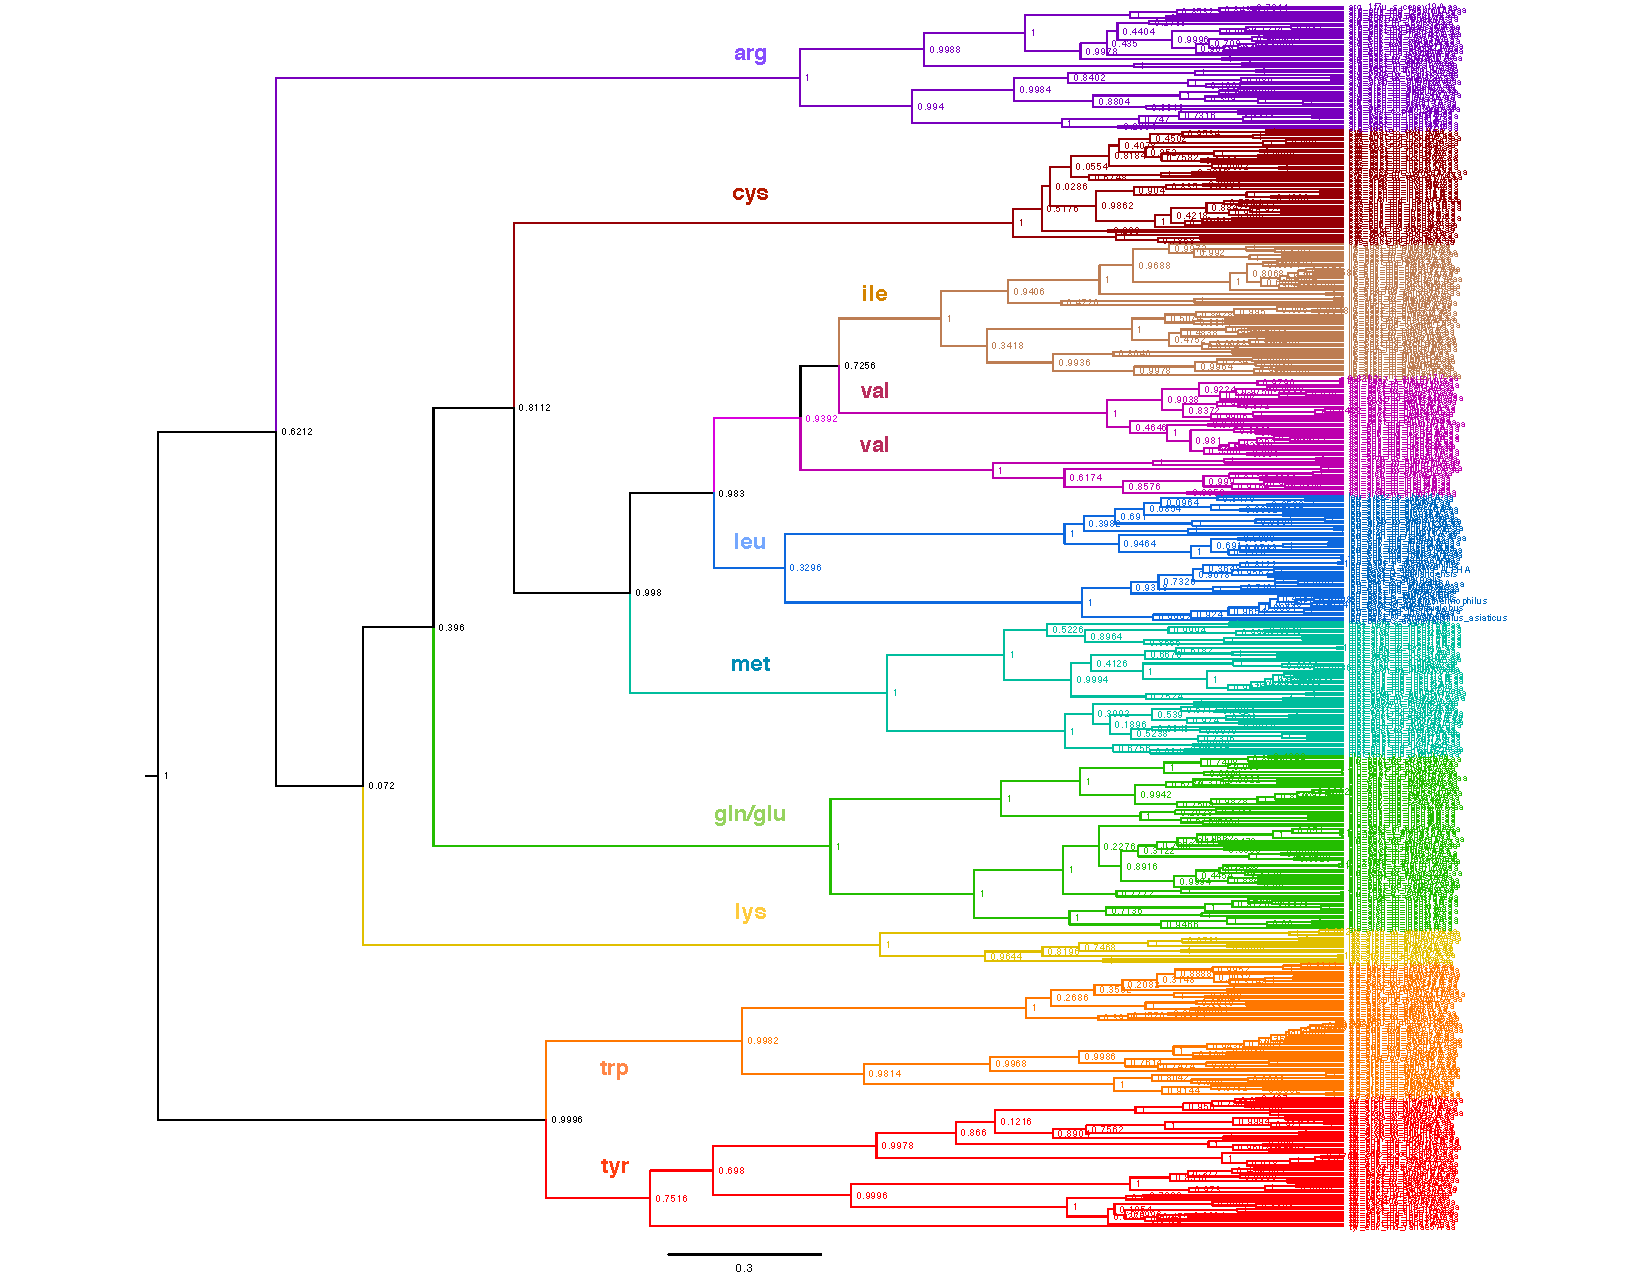
\includegraphics[width=\textwidth]{ClassI_Coalescent_1}
\end{figure}

% Either type in your references using
% \begin{thebibliography}{}
% \bibitem{}
% Text
% \end{thebibliography}
%
% or
%
% Compile your BiBTeX database using our plos2015.bst
% style file and paste the contents of your .bbl file
% here. See http://journals.plos.org/plosone/s/latex for 
% step-by-step instructions.
% 
\begin{thebibliography}{10}

% Use this sample article?? -could relate to Rodin-Ohno hypothesis

%\bibitem{bib1}
%G. C. Conant, K. H. Wolfe.
%\newblock {{T}urning a Hobby into a Job: How Duplicated Genes Find New
%  functions}.
%\newblock Nat Rev Genet. Dec;9(12):938--950. 2008.

% Woese paper
\bibitem{Woese} 
Woese CR, Olsen GJ, Ibba M, Soll D.
\newblock Aminoacyl-tRNA synthetases, the genetic code, and the evolutionary process.
\newblock Microbiology and Molecular Biology Reviews, p. 202-236. 2000.

% Malaria (prolyl-) paper
\bibitem{MalariaProlyl} 
Herman JD, Pepper LR, Cortese JF, Estiu G, Galinsky K, Zuzarte-Luis V, Derbyshire ER, Ribacke U, Lukens AK, Santos SA, Patel V, Clish CB, Sullivan Jr. WJ, Zhou H,
Bopp SE, Schimmel P, Lindquist S, Clardy J, Mota MM, Keller TL, Whitman M, Wiest O, Wirth DF, Mazitschek R. 
\newblock The cytoplasmic prolyl-tRNA synthetase of the malaria parasite is a dual-stage target of febrifugine and its analogs.
\newblock Science Translation Medicine, Vol 7, Issue 288. 2015.

% Previous aaRS phylogenies
\bibitem{aaRSphylogeny1999} 
Wolf YI, Aravind L, Grishin NV, Koonin EV.
\newblock Evolution of aminoacyl-tRNA synthetases--analyses of unique domain architectures and phylogenetic trees reveals a complex history of horizontal gene transfer events.
\newblock Genome Research, (8):689-710. 1999.

% Previous aaRS phylogenies
\bibitem{aaRSphylogeny2017} 
Chaliotis A, Vlastaridis P, Mossialos D, Ibba M, Becker HD, Stathopoulos C, Amoutzias GD.
\newblock The complex evolutionary history of aminoacyl-tRNA synthetases.
\newblock Nucleic Acids Research, 45(3):1059-1068. 2018. doi: 10.1093/nar/gkw1182.

% Modeller paper
\bibitem{Modeller}
Webb B, Sali A.
\newblock Comparative protein structure modeling using Modeller.
\newblock Current Protocols in Bioinformatics, John Wiley and Sons, Inc., 5.6.1-5.6.32. 2014.

% POSA paper 0
\bibitem{POSA}
Ye Y, Godzik A.
\newblock Multiple flexible structure alignment using partial order graphs.
\newblock Bioinformatics, vol. 21 (pg. 2362-2369). 2005.

% POSA paper 1
\bibitem{POSA1}
Li Z, Natarajan P, Ye Y, Hrabe T, Godzik A.
\newblock POSA: A user-driven, interactive multiple protein structure alignment server.
\newblock Nucl. Acids Res. 2014. doi: 10.1093/nar/gku394

% BEAST
\bibitem{BEAST}
Drummond AJ, Rambaut A.
\newblock BEAST: Bayesian evolutionary analysis by sampling trees.
\newblock BMC Evolutionary Biology. 2007. doi: 10.1186/1471-2148-7-214.

% BEAST 1.7
\bibitem{BEAST1point7}
Drummond AJ, Suchard MA, Xie Dong, Rambaut A.
\newblock Bayesian phylogenetics with BEAUti and the BEAST 1.7.
\newblock Molecular Biology and Evolution, 29(8): 1969-1973. 2012. doi: 10.1093/molbev/mss075.

% BEAST 2 paper
\bibitem{BEAST2}
Bouckaert R, Heled J, Kühnert D, Vaughan T, Wu C-H, Xie D, Suchard MA, Rambaut A, Drummond AJ.
\newblock BEAST 2: A software platform for Bayesian evolutionary analysis.
\newblock PLoS Computational Biology, 10(4), e1003537. 2014. doi: 10.1371/journal.pcbi.1003537

% HHpred paper
\bibitem{HHpred}
Söding J, Biegert A, Lupas AN.
\newblock The HHpred interactive server for protein homology detection and structure prediction. 
\newblock Nucleic Acids Research. 33(Web Server issue):W244-W248. doi: 10.1093/nar/gki408. 2005.

% Bayes theorem
\bibitem{Bayes}
Bayes, Price
\newblock An essay towards solving a problem in the doctrine of chances.
\newblock Philosophical Transactions of the Royal Society, 53:370-418. 1763. doi:10.1098/rstl.1763.0053

% Stats guide for biologists
\bibitem{ConfidenceInterval}
Nakagawa S, Cuthill IC.
\newblock Effect size, confidence interval and statistical significance: a practical guide for biologists.
\newblock Biological Reviews, 82(4): 591-605. 2007. doi: 10.1111/j.1469-185X.2007.00027.x.

% Prior and posterior in Bayesian phylogenetics
\bibitem{PPinBayesianPhylogenetics}
Alfaro ME, Holder MT.
\newblock The posterior and the prior in Bayesian phylogenetics.
\newblock Annual Review of Ecology, Evolution, and Systematics, 37: 19-42. 2006. doi: 10.1146/annurev.ecolsys.37.091305.110021

% Bayesian phylogenetics
\bibitem{Huelsenbeck} 
Huelsenbeck JP, Ronquist F, Nielsen R, Bollback JP.
\newblock Bayesian inference of phylogeny and its impact on evolutionary biology.
\newblock Science, 294(5550):2310-2314. 2001. doi: 10.1126/science.1065889

% Bayesian phylogenetics
\bibitem{HolderLewis} 
Holder M, Lewis PO.
\newblock Phylogeny estimation: traditional and Bayesian approaches.
\newblock Nature Reviews Genetics, 4:275-284. 2003. doi: 10.1038/nrg1044

%%%%
% BAYESIAN PHYLOGENETICS PAPERS

% Science, explicit 'Bayesian phylogenetics' in title
\bibitem{MammalRadiation} 
Murphy WJ, Eizirik E, O'Brien SJ, Madsen O, Scally M, Douady CJ, Teeling E, Ryder OA, Stanhope MJ, de Jong WW, Springer MS.
\newblock Resolution of the early placental mammal radiation using Bayesian phylogenetics.
\newblock Science, 294(5550): 2348-2351. 2001. doi: 10.1126/science.1067179

% Early mammal evolution
\bibitem{EarlyMammals} 
Jow H, Hudelot C, Rattray M, Higgs PG.
\newblock Bayesian phylogenetics using an RNA substitution model applied to early mammalian evolution.
\newblock Molecular Biology and Evolution, 19(9): 1591-1601. 2002. doi: 10.1093/oxfordjournals.molbev.a004221

% Missing data no problem for Bayesian phylogenetics
\bibitem{MissingData} 
Wiens JJ, Moen DS.
\newblock Missing data and the accuracy of Bayesian phylogenetics.
\newblock Journal of Systematics and Evolution, 46(3): 307-314. 2008. doi: 10.3724/SP.J.1002.2008.08040.

% SPREAD
\bibitem{SPREAD} 
Bielejec F, Rambaut A, Suchard MA, Lemey P.
\newblock SPREAD: spatial phylogenetic reconstruction of evolutionary dynamics.
\newblock Bioinformatics, 27(20): 2910-2912. 2011. doi: 10.1093/bioinformatics/btr481.

% Mammal diversification
\bibitem{MammalDiversification}
Meredith, Janecka JE, Gatesy J, Ryder OA, Fisher CA, Teeling EC, Goodbla A, Eizirik E, Simao TLL, Stadler T, Rabosky DL, Honeycutt RL, Flynn JJ, Ingram CM, Steiner C, Williams TL, Robinson TJ, Burk-Herrick A, Westerman M, Ayoub NA, Springer MS, Murphy WJ.
\newblock Impacts of the Cretaceous terrestrial revolution and KPg Extinction on mammal diversification.
\newblock Science, 334(6055): 521-524. 2011. doi: 10.1126/science.1211028.

% Sampled ancestors
\bibitem{SampledAncestors}
Gavryushkina A, Heath TA, Ksepka DT, Stadler T, Welch D, Drummond AJ.
\newblock Bayesian total-evidence dating reveals recent crown radiation of penguins.
\newblock Systematic Biology, 66(1): 57-73. 2016. doi: 10.1093/sysbio/syw060.

% Phylodynamics
\bibitem{Phylodynamics}
Rasmussen DA, Kouyos R, Gunthard HF, Stadler T.
\newblock Phylodynamics on local sexual contact networks.
\newblock PLOS Computational Biology. 2017. doi: 10.1371/journal.pcbi.1005448.

%%%%

% Relaxed clock model selection 
\bibitem{RelaxedClockModelSelection} 
Baele G, Li WLS, Drummond AJ, Suchard MA.
\newblock Accurate model selection of relaxed molecular clocks in Bayesian phylogenetics.
\newblock Molecular Biology and Evolution, 30(2): 239-243. 2013. doi: 10.1093/molbev/mss243

% Maximum likelihood 
\bibitem{Guindon}
Guindon S, Gascuel O.
\newblock A simple, fast, and accurate algorithm to estimate large phylogenies by maximum likelihood.
\newblock Systematic Biology, 52(5):696-704. 2003. doi: 10.1080/10635150390235520

% 
\bibitem{bib2}
Marti-Renom MA, Stuart A, Fiser A, Sánchez R, Melo F, Sali A. 
\newblock Comparative protein structure modeling of genes and genomes.
\newblock Annual Review of Biophysics and Biomolecular Structure. 29, 291-325. 2000.

%
\bibitem{bib3}
Sali A, Blundell TL.
\newblock Comparative protein modelling by satisfaction of spatial restraints.
\newblock J. Mol. Biol. 234, 779-815. 1993.

% 
\bibitem{bib4}
Fiser A, Do RK, Sali A.
\newblock Modeling of loops in protein structures.
\newblock Protein Science 9. 1753-1773. 2000.

% MCMC paper
\bibitem{MCMC}
Drummond AJ, Nicholls GK, Rodrigo AG, Solomon S. 
\newblock Estimating mutation parameters, population history and genealogy simultaneously from temporally spaced sequence data.
\newblock Genetics 161, 1307-1320. 2002.

% Metropolis
\bibitem{Metropolis}
Metropolis N, Rosenbluth A, Rosenbluth M, Teller A, Teller E.
\newblock Equations of state calculations by fast computing machines.
\newblock Journal of Chemical Physics, 21(6): 1087-1091. 1953. doi: 10.1063/1.1699114.

% Hastings
\bibitem{Hastings}
Hastings WK.
\newblock Monte Carlo sampling methods using Markov chains and their applications.
\newblock Biometrika, 57(1): 97-109. 1970. doi: 10.2307/2334940.

% MCMC efficiency
\bibitem{MCMCefficiency}
Lakner C, van der Mark P, Huelsenbeck JP, Larget B, Ronquist F.
\newblock Efficiency of Markov chain Monte Carlo tree proposals in Bayesian phylogenetics.
\newblock Systematic Biology, 57(1): 86-103. 2008. doi: 10.1080/10635150801886156.

% Wills paper - Emergence of Coding (intro to Remco's method)
\bibitem{bib11} 
Wills PR, Nieselt K, McCaskill JS.
\newblock Emergence of coding and its specificity as a physico-informatic problem.
\newblock Origins of Life and Evolution of Biospheres. 2015. doi: 10.1007/s11084-015-9434-5.

% Rodin-Ohno paper
\bibitem{RodinOhno} 
Rodin SN, Ohno S.
\newblock Four primordial modes of tRNA-Synthetase recognition, determined by the (G,C) operational code.
\newblock Proceedings of the National Academy of Sciences, Vol 94, pp. 5183-5188. 1997.

% Rodin-Ohno-Rodin paper
\bibitem{RodinOhnoRodin} 
Rodin S, Ohno S, Rodin A.
\newblock Transfer RNAs with complementary anticodons: Could they reflect early evolution of discriminative genetic code adaptors?
\newblock Proceedings of the National Academy of Sciences, Vol 90, pp. 4723-4727. 1993.

% BOOK - CHECK CITATION FORMAT
\bibitem{bib13} 
Ibba M, Francklyn C, Cusack S.
\newblock The aminoacyl-tRNA synthetases.
\newblock Molecular Biology Intelligence Unit, Landes Bioscience. Georgetown, Texas, U.S.A. 2005.

% Molecular clock paper (longer time leads to genetic saturation)
\bibitem{bib14} 
Ho SY, Phillips MJ, Cooper A, Drummond AJ.
\newblock Time dependency of molecular rate estimates and systematic overestimation of recent divergence times.
\newblock Molecular Biological Evolution, 7:1561-8. 2005. doi: 10.1093/molbev/msi145.

% Molecular clock paper (relaxed clock)
\bibitem{bib15} 
Drummond AJ, Ho SYW, Phillips MJ, Rambaut A.
\newblock Relaxed phylogenetics and dating with confidence.
\newblock PLoS Biology, 4(5):e88. 2012. doi: 10.1073/pnas.1207965110.

% BDSKY paper
\bibitem{BDSKY} 
Stadler T, Kuhnert D, Bonhoeffer S, Drummond AJ.
\newblock Birth-death skyline plot reveals temporal changes of epidemic spread in HIV and hepatitis C virus (HCV).
\newblock Proceedings of the National Academy of Sciences of the United States of America, 110(1):228-33. 2013. doi: 10.1073/pnas.1207965110.

% Coalescent skyline paper
\bibitem{coalSky} 
Drummond AJ, Rambaut A, Shapiro B, Pybus OG.
\newblock Bayesian coalescent inference of past population dynamics from molecular sequences.
\newblock Molecular Biology and Evolution, 22(5): 1185-92. 2005. doi: 10.1093/molbev/msi103


%%%%
% BAYESIAN CRITICS

% Overcredibility
\bibitem{Overcredibility} 
Suzuki Y, Glazko GV, Nei M.
\newblock Overcredibility of molecular phylogenies obtained by Bayesian phylogenetics.
\newblock Proceedings of the National Academy of Sciences of the United States of America, 99(25): 16138-16143. 2002. doi: 10.1073/pnas.212646199.

% Model assumptions
\bibitem{ModelAssumption} 
Lemmon AR, Moriarty EC, Sullivan J.
\newblock The importance of proper model assumption in Bayesian phylogenetics.
\newblock Systematic Biology, 53(2): 265-277. 2004. doi: 10.1080/10635150490423520.

% Data partitioning and Bayes factors
\bibitem{BF} 
Brown JM, Lemmon AR, Jockusch E.
\newblock The importance of data partitioning and the utility of Bayes factors in Bayesian phylogenetics.
\newblock Systematic Biology, 56(4): 643-655. 2007. doi: 10.1080/10635150701546249.

%%%%

\end{thebibliography}


\end{document}

